\section{Introduction}
\label{sec:intro}

\begin{figure}[!th]
     \centering    
    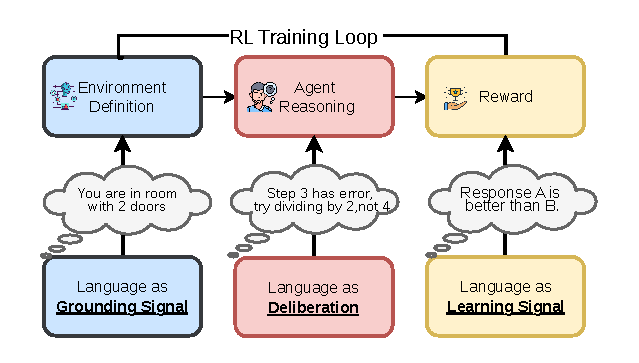
\includegraphics[width=1.1\linewidth]{paper_images/main_figure.pdf}
   \caption{\footnotesize  Language plays three complementary roles in agent's development lifecycle: grounding the environment, scaffolding intermediate reasoning, and providing learning signal for further training.}
    \label{fig:VRLrepresentation}
\end{figure}


\begin{figure*}[!th]
    \centering    
    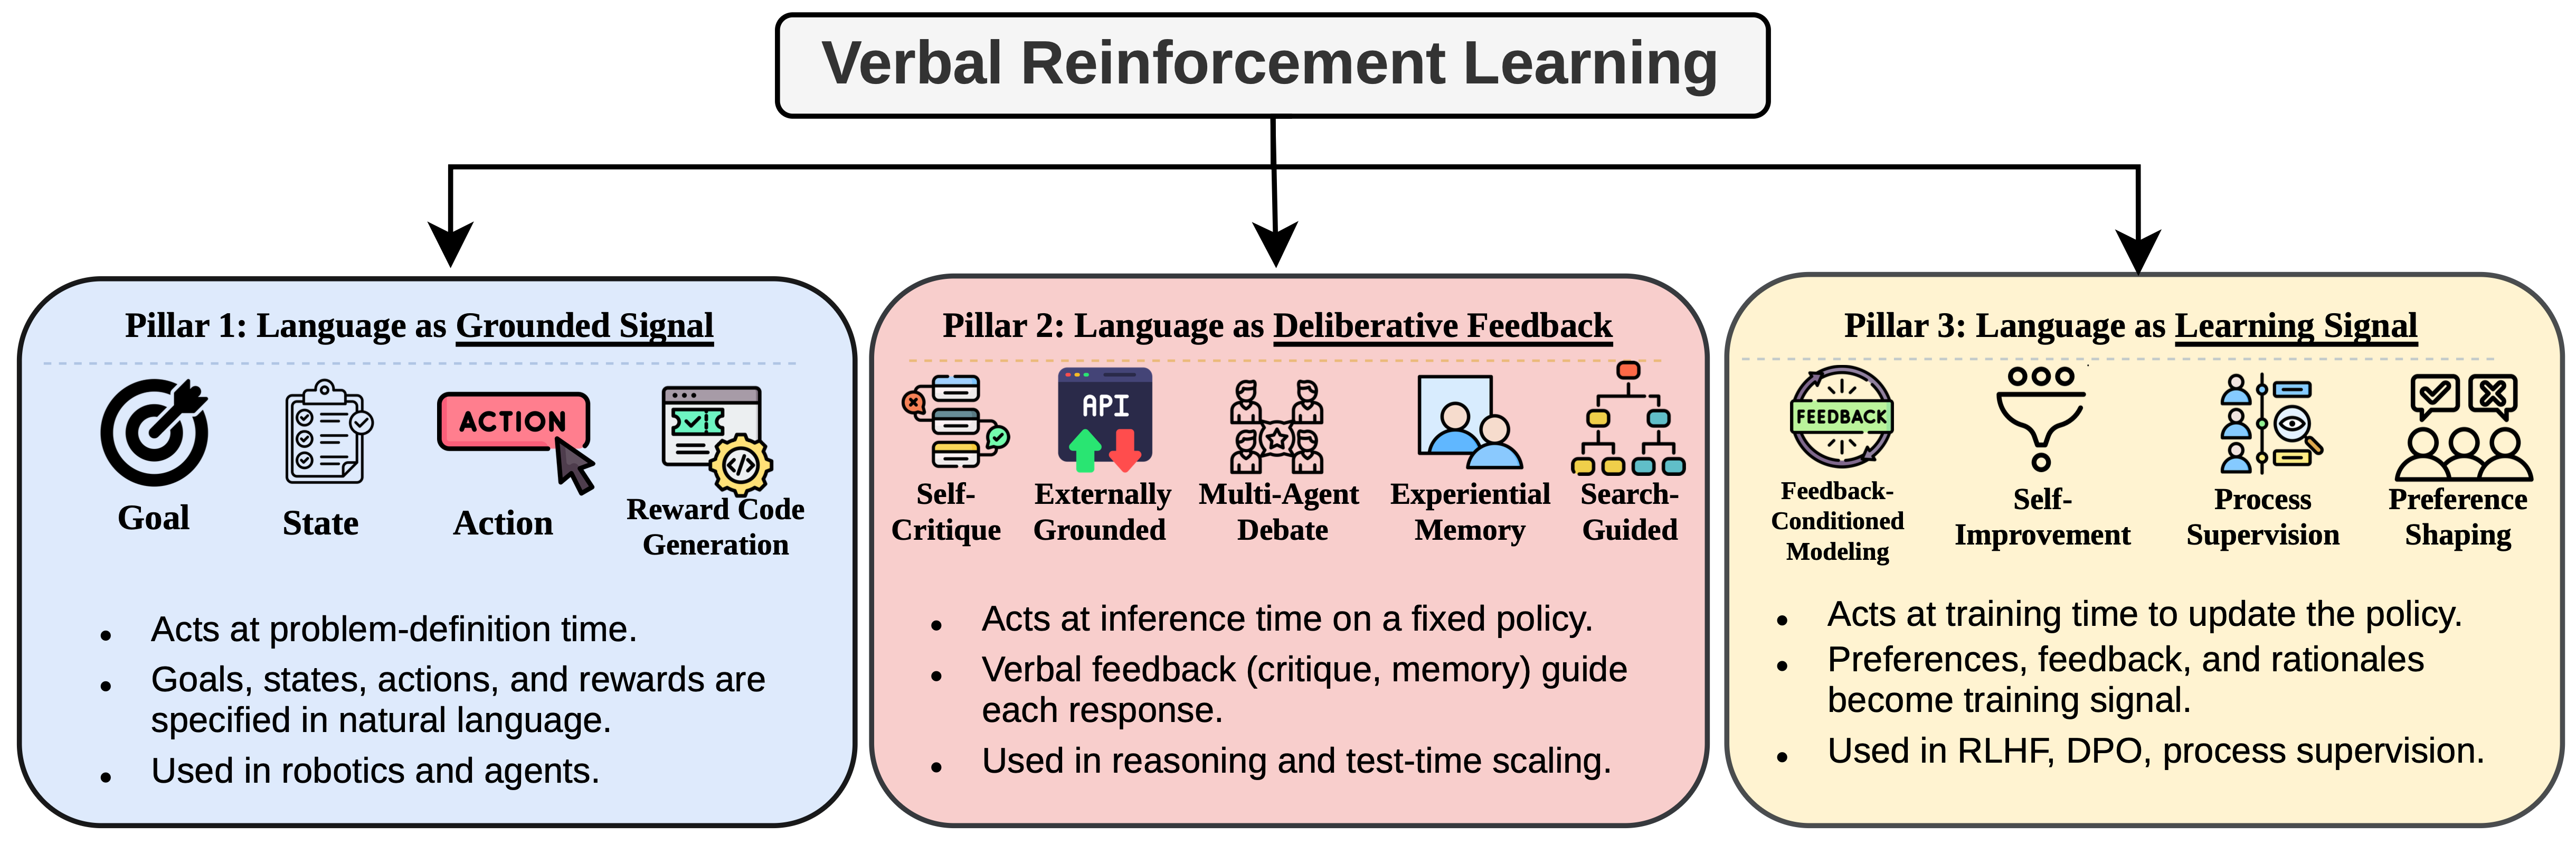
\includegraphics[width=\textwidth]{paper_images/Figure-2-new.png}
    \caption{\footnotesize Our proposed taxonomy of Verbal Reinforcement Learning. Language serves three distinct functional roles: \textit{grounding signal}, which structures environment interaction; \textit{deliberative feedback}, which operates at inference time to refine reasoning; and \textit{learning signal}, which drives parameter updates at training time.
    }
    \label{fig:taxonomy}
\end{figure*}

% Describe shortcoming on canonical reinforcement learning
Classical reinforcement learning has achieved remarkable successes by coupling agents with well-specified environments, action spaces, reasoning mechanisms, and task-specific reward functions. This framework has enabled agents to master Atari games \citep{mnih2015human}, defeat world champions at Go \citep{silver2016mastering}, optimize chip placement \citep{mirhoseini2021graph}, and control complex physical systems \citep{degrave2022magnetic}. However, each success rests on heavy domain-specific engineering: the environment must be formalized, the interaction space defined, and the reward function must closely capture the intended behavior \citep{vamplew2021scalarrewardenoughresponse}. Designing such specifications is a long-standing bottleneck \citep{amodei2016concrete}, especially in settings where tasks and goals are ambiguous, context-dependent, and difficult to encode directly.



The emergence of large language models \citep{brown2020language} has introduced an alternative supervisory channel: natural language. Instead of requiring all task intent to be predefined, verbal feedback enables on-the-fly communication of corrections, preferences, and constraints in a manner that agents are increasingly able to interpret and implement. Modern large language models, particularly frontier models \citep{achiam2023gpt}, can accurately describe a wide range of phenomena. These capabilities include describing environments \citep{wang2023voyager}, identifying bugs in code \citep{mcaleese2024criticgpt}, critiquing generated outputs \citep{madaan2023selfrefine}, and translating human preferences into actionable training signals \citep{hong2024orpo, meng2024simpo}. Similar to how self-supervised learning \citep{devlin2019bertpretrainingdeepbidirectional, chen2020simple} expanded the use of unlabeled data in model development, verbal feedback is emerging as an important source of supervision for language-model-based agents. 




We refer to this family of methods as \textbf{Verbal Reinforcement Learning (VRL)}\removed{: \textit{a paradigm in which an agent receives natural-language feedback---whether self-generated, provided by a human, or produced by an external tool or model---and uses it to improve its behavior and guide future decision-making}. Feedback may be used directly as text or converted into a compressed training signal for parameter updates.}\added{, and we define it by two inclusion criteria: \textit{(i) the feedback is expressed in natural language, whether self-generated, provided by a human, or produced by an external tool or model, and its linguistic structure is functionally consumed by the agent, rather than being collapsed to a scalar or preference bit before use; and (ii) the feedback participates in an improvement loop, that is, an output revision, a memory write, or a parameter update.} Both criteria are required, and they fence VRL off from adjacent paradigms. Plain instruction following satisfies neither, since no improvement loop exists. Vanilla RLHF and DPO satisfy only the second, because the verbal judgment is reduced to a preference bit before learning; we discuss them only as the scalar endpoint of the compression spectrum in Section~\ref{sec:pillar3}. Language-conditioned RL treats language as an input to the policy rather than as feedback on its behavior. One boundary case the criteria settle: language consumed at specification time to construct a reward function, as in reward-code generation, satisfies criterion (i) even though the constructed function later emits scalars.} The term was introduced by \citet{shinn2023reflexion} to describe self-reflective agents (specific instance of what we call deliberative feedback); \removed{here, it is adopted more broadly to encompass any method in which verbal feedback shapes an agent's outputs, learned policy, or problem specification.}\added{we deliberately generalize it to any method meeting the two criteria above, and we state this generalization explicitly to avoid conflation with the original, narrower sense.}
 

Early results demonstrate that verbal feedback can drive substantial improvements across diverse settings. \citet{ahn2022can} used language to ground high-level instructions in physical affordances, enabling real-world robotic planning. \citet{shinn2023reflexion} achieved 91\% pass@1 on HumanEval through verbal self-reflection alone, and \citet{madaan2023selfrefine} showed that iterative verbal critique yields substantial gains across diverse generation tasks. \citet{ouyang2022training} demonstrated that a 1.3B-parameter model trained on verbal preference judgments outperformed the 175B GPT-3 baseline, a 130$\times$ size disadvantage overcome by richer supervision. These are not isolated demonstrations and publications on arXiv referencing ``self-refine,'' ``self-correction,'' ``verbal feedback,'' and ``language-feedback alignment'' have grown from a handful in early 2020 to several hundred today, spanning multiple domains including coding assistants \citep{yang2024swe, jimenez2024swebenchlanguagemodelsresolve}, scientific discovery \citep{m2024augmenting, lu2024ai}, robotics \citep{wang2023voyager}, mathematical reasoning \citep{hatamizadeh2026igrpo, liu2026dual, shi2025ssr}, clinical decision-making \citep{huang2025medreflect, zhou2025enhancing} and education \citep{qian2025dean, ahtisham2026ai}.



These methods differ in their mechanisms (Figure~\ref{fig:VRLrepresentation}): some operate during inference, others modify training data, and some redefine the task itself . However, they share a common characteristic: the use of natural language to guide, refine, and ground agent behavior. Yet no existing framework unifies them. Prior surveys have examined language-conditioned policies in text-based environments \citep{luketina2019survey}, the bidirectional synergies between LLMs and RL \citep{pternea2024rl}, LLM self-correction in isolation \citep{kamoi2024can}\added{, automatic correction strategies \citep{pan2023automatically}, feedback integration for text generation \citep{fernandes2023bridging}, preference optimization \citep{kaufmann2023survey, xiao2024comprehensive}, agent memory \citep{zhang2025survey}, test-time scaling \citep{zhang2025testtime}, self-evolving agents \citep{gao2025selfevolving, fang2025selfevolving}, and reinforcement learning for LLM agents \citep{zhang2025agenticrl}; Natural Language Reinforcement Learning \citep{feng2024natural} recasts RL components in language space but is a framework proposal rather than a survey. Table~\ref{tab:surveys} in Appendix~\ref{app:surveys} positions our taxonomy against these works: they organize by mechanism or by agent capability, whereas we organize by the signal itself}. In contrast, our survey focuses on the functional role of \emph{verbal feedback} as a first-class signal for improving agent, organized along a single axis: \emph{when} natural language enters the agent's lifecycle and \emph{what} it modifies. We formalize this axis into a three-pillar taxonomy in Section~\ref{sec:taxonomy}. This paper makes following contributions:

 \begin{itemize}

    \item We present the first comprehensive survey of Verbal Reinforcement Learning, \removed{defining the paradigm broadly}\added{defining the paradigm through explicit inclusion criteria that separate it from RLHF, instruction following, and language-conditioned RL,} and proposing a three-pillar taxonomy (Section~\ref{sec:taxonomy}) that organizes the field by \emph{when} language acts in the agent lifecycle.
    \item Within each pillar, we synthesize representative methods, identify cross-cutting challenges and outline future directions for developing robust, capable and aligned Verbal RL agents.
    \item \added{We give explicit decision rules for methods whose signals span pillars, including a hybrid-cases table (Table~\ref{tab:hybrid}), so the taxonomy is applicable rather than merely descriptive.}
    \item \added{We distill practitioner guidance for choosing among verbal-feedback mechanisms (Appendix~\ref{app:guide}) and position the survey against prior overviews (Appendix~\ref{app:surveys}).}



    % \item We propose a taxonomy organized by the functional role of language in the agent lifecycle: deliberative feedback (test-time), learning signal (train-time), and grounding signal (problem definition). \das{should we say someting about novelty, should we highlight that we have broadened the definition of verbal LM from Shinn et.al. 2023?}
    % \item We survey representative papers under each pillar and further identify subcategories, identifying both their methodologies and conceptual contributions. \das{maybe we need to say something like why this is useful , also is it subcategory or themes?}
    % \item We explore emerging applications, provide insights and outline a roadmap for developing more capable and aligned agents. \das{this again is too vague, we need to say to what degree or why they are capable and aligned}
\end{itemize}

We organize the paper as follows. Section~\ref{sec:taxonomy} introduces the three-pillar taxonomy and a working example showing how the pillars operate together in a single coding agent. Sections~\ref{sec:pillar1}--\ref{sec:pillar3} develop each pillar of the taxonomy in detail: language as grounding signal, as deliberative feedback, and as learning signal, respectively. Finally, section~\ref{sec:discussion} presents cross-cutting insights and outlines future research directions, while section~\ref{sec:conclusion} provides the conclusion.


% Although the idea of using natural-language feedback to improve language agents has gained momentum only in the last few years, there is already a rapidly growing body of work on this topic. A search on arXiv for terms such as ``self-refine,'' ``self-correction,'' ``verbal feedback,'' and ``language-feedback alignment'' shows publications growing from a handful in 2020 to several hundreds now. This work is being pursued across diverse application domains, including coding assistants \citep{yang2024sweagent, jimenez2024swebench}, scientific discovery \citep{mbran2024chemtools, lu2024aiscientist}, robotics \citep{ahn2022can, wang2023voyager}. Early results are promising: language agents have reached 91\% pass@1 on HumanEval through verbal self-reflection alone \citep{shinn2023reflexion}; a 1.3B-parameter InstructGPT model trained from preference-based language feedback outperformed the 175B GPT-3 baseline \citep{ouyang2022training}; and iterative self-critique has yielded substantial gains across diverse generation tasks \citep{madaan2023selfrefine}.

% A growing body of work treats natural language as part of the agent-improvement loop, spanning the three regimes our taxonomy later formalizes. At problem-definition time, \citet{ahn2022can} used language to ground high-level instructions in physical affordances for real-world robotic planning. At inference time, \citet{madaan2023selfrefine} showed that iterative verbal feedback yields substantial improvements across diverse generation tasks. At training time, \citet{ouyang2022training} showed that a 1.3B-parameter InstructGPT model trained from verbal preference judgments outperformed the 175B GPT-3 model. These methods differ in mechanism but share a common pattern: natural language is used to guide, refine and ground agent behavior. Consider a single coding agent that resolves a GitHub issue: a natural-language issue description defines the task, execution traces and error messages guide its iteration, and successful trajectories train the next model. The same agent consumes verbal feedback at three distinct timescales, each producing a different effect. No existing framework unifies these regimes, which is what this survey provides. The goal of this survey is to bring these developments to the broader ML community, to make researchers aware of the progress that has been made, and to surface the gaps and opportunities that exist for advancing research in this promising direction. 




% The canonical reinforcement learning framework is defined by an agent that perceives states, takes actions, and receives scalar reward signals. This approach has taught agents to master Atari from raw pixels \citep{mnih2015human}, defeat world champions at Go \citep{silver2016mastering}, design the chip layouts inside production accelerators \citep{mirhoseini2021graph}, and stabilize the superheated plasma inside a tokamak fusion reactor in real time \citep{degrave2022magnetic}, \das{are these common examples?} among many others. Each of these successes, however, rests on carefully designing a scalar reward signal. However, \das{two consequetive howevers} designing correct signal is hard \citep{vamplew2021scalarrewardenoughresponse} and the signal itself is  sparse and vulnerable to reward hacking \citep{amodei2016concrete}. 
% \das{if you say for example after the previous sentence, it will mean that you are exemplifying why designing correct signal is hard. Instead, below you are just contrasting scalar number with what a llm can generate, but not proving the above point. Consider rewrtiting the sentences below. }
% For example, if a robotic agent drops a cup, it will receive a negative reward. A human supervisor, by contrast, might say, ``You gripped it too firmly near the rim---try a broader, softer grasp.'' That verbal feedback carries causal structure, corrective direction, and domain knowledge that no scalar value can express.



% Emergence of large language model and defining the term verbal reinforcement learning

% With the proliferation of large language models \citep{brown2020language}, particularly frontier models \citep{anderljung2023frontier}, \das{this is a weird citation. also for this and the previous one you could technically cite a lot of sota model papers } the generation of nuanced and accurate verbal feedback at scale has become increasingly feasible. These models can describe environments \citep{wang2023voyager}, identify bugs in code \citep{mcaleese2024criticgpt}, reason about logical structure, and critique or refine generated outputs \citep{madaan2023selfrefine}. Just as self-supervised \citep{devlin2019bertpretrainingdeepbidirectional,chen2020simple} learning unlocked a new era of progress by freeing models from the bottleneck of labeled data, verbal feedback from LLMs has emerged as the primary engine \das{should we say something less bold, its not the only way to get improvements though } of improvement for language-model-based agents\das{on what?}. 
% % The pattern is striking in its symmetry: models now generate their own feedback/instructions and consume it to improve themselves \citep{yuan2025selfrewarding}, closing the loop with minimal or no human intervention. 
% We refer to this family of methods as \textbf{Verbal Reinforcement Learning} (\verbalrl). The term was introduced by \citet{shinn2023reflexion} to describe
% self-reflective agents\das{does this mean they primarily focused on the deliberative feedback part? if yes then we can make it clear and also say what that means}; we adopt it more broadly to encompass any
% paradigm in which an agent receives natural-language feedback,
% whether self-generated, provided by humans, or sourced from
% external tools and models, and uses it to improve its policy
% and guide future decision-making.


% The rise of verbal feedback is marked with the proliferation of large language models \citep{brown2020language}, which make it increasingly feasible to generate, interpret, and act on natural-language feedback at scale. Such models can describe environments \citep{wang2023voyager}, identify bugs in code \citep{mcaleese2024criticgpt}, critique generated outputs \citep{madaan2023selfrefine}, and translate human preferences or corrections into forms that agents can use. Just as self-supervised learning \citep{devlin2019bertpretrainingdeepbidirectional,chen2020simple} expanded the role of unlabeled data in model development, verbal feedback is emerging as an important source of supervision for language-model-based agents. 

% This shift has been enabled by advancement of large language models \citep{brown2020language}, which can now generate verbal feedback at scale. Such models can describe environments \citep{wang2023voyager}, identify bugs in code \citep{mcaleese2024criticgpt}, critique generated outputs \citep{madaan2023selfrefine}, and translate human preferences into forms that agents can use. Just as self-supervised learning \citep{devlin2019bertpretrainingdeepbidirectional,chen2020simple} freed model development from the bottleneck of labeled data, verbal feedback is freeing agent improvement from the bottleneck of design soecification.We refer to this family of methods as \textbf{Verbal Reinforcement Learning (VRL)}: \textit{a paradigm in which an agent receives natural-language feedback---whether self-generated, provided by a human, or produced by an external tool or model, to improve its behavior and guide future decision-making}. The feedback, could be used directly as text or after conversion into a compressed training signal. Based on when the feedback takes effect in agent's lifecycle, we define our taxonomy of verbal feedback methods along a single axis: \emph{when} natural language enters the agent's lifecycle and, consequently, yielding three pillars i.e. language as grounding signal, language as deliberative feedback and language as learning signa. The term VRL was introduced by \citet{shinn2023reflexion} to describe self-reflective agents (specific instance of what we call deliberative feedback). We adopt the term more broadly to encompass methods in which verbal feedback shapes the agent's outputs, policy, or problem specification. This survey makes three primary contributions:

% ================================================

% Although verbal RL scales easily, incorporating verbal language into an RL model is a hard, challenging problem. The reason being is these verbals 


% % Challenges and Open Questions
% Integrating verbal feedback into the agent loop introduces challenges that cut across all three pillars. First, the faithfulness of verbal feedback is not guaranteed: when models generate their own critiques or reflections, these can be superficially plausible yet factually incorrect, leading the agent to learn from flawed diagnoses \citep{huang2023large}. Second, credit assignment becomes harder, not easier, with richer feedback — a verbal critique such as the response lacks depth and contains factual errors conflates multiple failure modes without precisely attributing them to specific decisions in the agent's trajectory. Third, when the same model generates both behavior and feedback, there is a risk of feedback collapse: the model preferentially reinforces outputs that align with its own distributional biases, gradually narrowing the policy in ways that mirror classical reward hacking \citep{saunders2022self}. Fourth, evaluation remains fragmented — methods operating at different stages of the agent loop are benchmarked on incommensurable tasks, making cross-pillar comparison difficult and obscuring which forms of verbal feedback yield the greatest improvement. A central goal of this survey is to surface these shared challenges, trace how they manifest differently across the three pillars, and identify the methodological gaps that future work must address.






% \begin{figure*}[t]
%     \centering
%     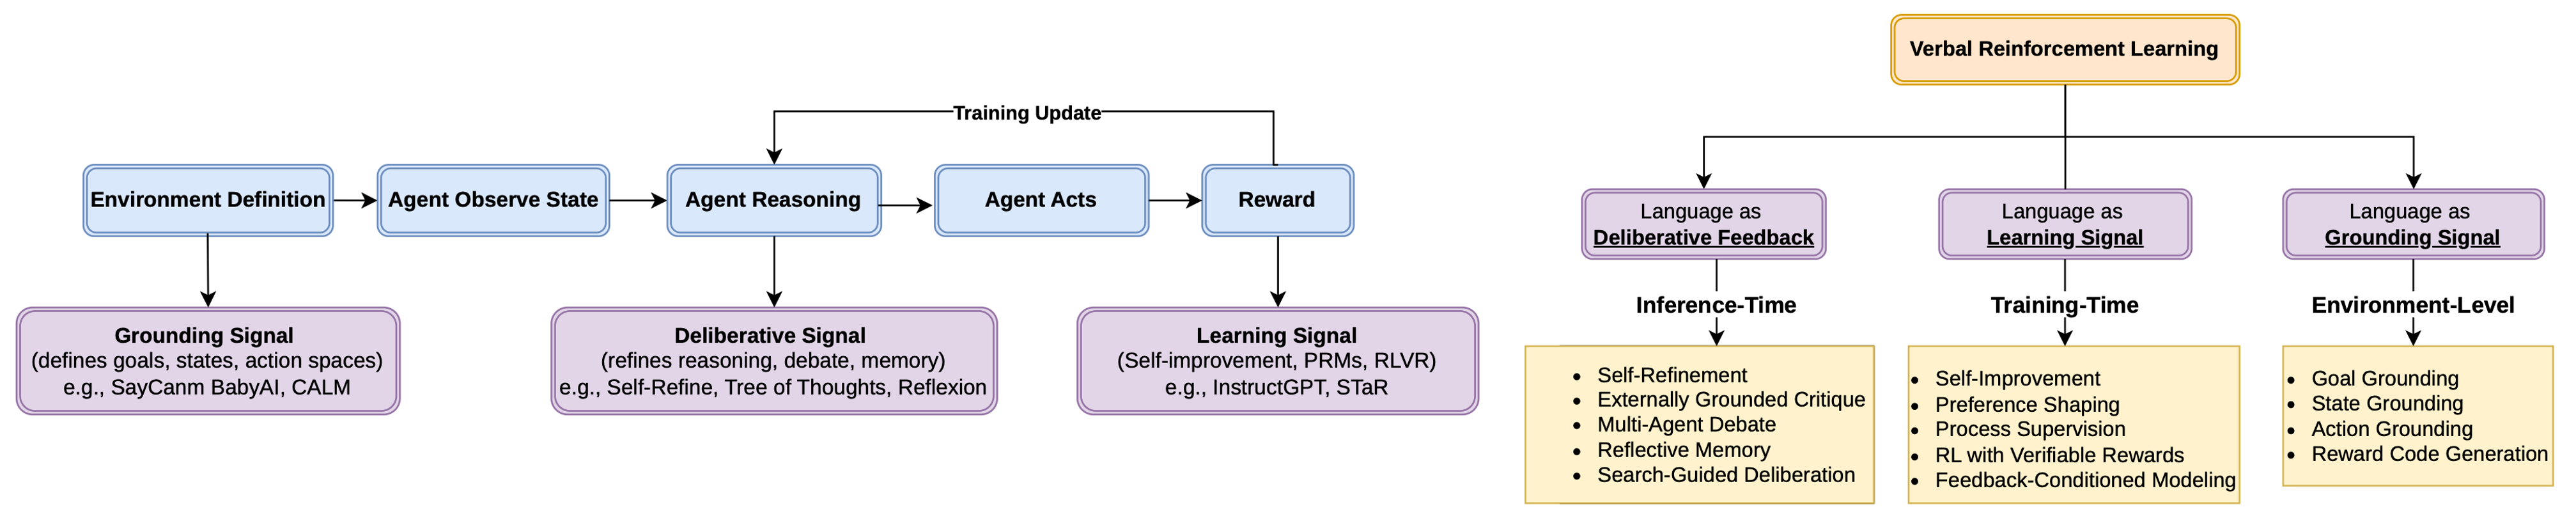
\includegraphics[width=\textwidth]{paper_images/Figure-7.png}
%     \caption{Your caption here.}
%     \label{fig:wide}
% \end{figure*}

% Describe our contribution


%scope of survey
% Our work complements \citep{luketina2019survey}, who focused on  language-conditioned policies in text-based environments; since then, the emergence of powerful LLMs has shifted language from conditioning input to an active computational substrate. Recent works like \citep{pternea2024rl} 
% examine the bidirectional potential of LLMs and RL,
% while \citet{kamoi2024can} specifically survey self-correction, a subset of our Pillar~1.  In contrast, our
% survey focuses on the functional role of \emph{verbal feedback} and how its being used to improve agent policy. 


% \das{i read the introduction, as a reader i still dont think its defined anywhere what verbal RL is lucidly.}


% The focus of this survey is on approaches that use verbal feedback as a first-class signal for improving language agents, where the feedback is explicit and central to the agent's improvement process. This distinguishes our survey from related works that focus on language-conditioned policies in text-based environments \citep{luketina2019survey}, the bidirectional synergies between LLMs and RL \citep{pternea2024rl}, LLM self-correction \citep{kamoi2024can}, or reinforcement learning from human feedback in isolation \citep{kaufmann2023survey}. Our survey creates a novel taxonomy that organizes verbal reinforcement learning along a single axis (\emph{when} language enters the agent lifecycle and \emph{what} it modifies), yielding three pillars: language as a grounding signal, language as deliberative feedback, and language as a learning signal.
 


% We organize the article as follows. Section~\ref{sec:taxonomy} introduces the three-pillar taxonomy and a worked example showing how the pillars operate together in a single coding agent. Section~\ref{sec:pillar1} discusses language as a grounding signal, with subcategories for goal grounding, state grounding, action grounding, and reward code generation. Section~\ref{sec:pillar2} surveys language as deliberative feedback, covering self-critique, externally grounded critique, multi-agent debate, experiential memory, and search-guided deliberation. Section~\ref{sec:pillar3} examines language as a learning signal, organizing methods along a compression spectrum from feedback-conditioned modeling to preference shaping. Finally, Section~\ref{sec:discussion} discusses cross-cutting insights and future research directions, and Section~\ref{sec:conclusion} concludes.